\documentclass[
    notheorems,
    11pt,
    compress,
    aspectratio=169
]{beamer}

\mode<presentation>{
    \usetheme{Madrid}
    \usecolortheme{orchid}
    \usefonttheme[onlymath]{serif}
    \setbeamertemplate{blocks}[rounded][shadow=true]
    \setbeamertemplate{navigation symbols}{}
    \setbeamertemplate{enumerate items}[square]
}

\usepackage{config}
\usepackage{soul}

\graphicspath{{./figures/}}
\bibliography{bibliography.bib}

% -----

\title[Introduzione all'Intelligenza Artificiale]{Intelligenza Artificiale e Machine Learning}
\subtitle{Introduzione all'Intelligenza Artificiale}
\author{prof. Leonardo Essam Dei Rossi}
\institute[]{ITT "M. Buonarroti" - Trento (TN)}
\date[A.S. 2025/2026]{Anno scolastico 2025/2026}

% -----

\begin{document}

\setlength{\baselineskip}{15pt}

\begin{frame}
    \titlepage
\end{frame}

\only<presentation>{
    \begin{frame}{Licenze e crediti}
        Questo materiale è disponibile sul sito Web del docente per il corso di \href{https://leonardodeirossi.github.io/teaching/2025-5inb-5inc-projectmanagement.html}{\structure{Gestione progetto e organizzazione d'impresa}} per gli studenti e le studentesse dell'anno scolastico 2025/2026.

        \vspace{\baselineskip}

        \begin{tabular}{@{}l l@{}}
            \textbf{Versione:} & \texttt{1.0.0}
            \\
            \textbf{Ultima modifica:} & 11/03/2026 20:27
        \end{tabular}

        % \vspace{\baselineskip}

        \vfill
        
        \begin{columns}
            \column{0.7\textwidth}
                \vfill
                This work is licensed under a \href{https://creativecommons.org/licenses/by-nc-sa/4.0/}{\structure{Creative Commons Attribution-NonCommercial-ShareAlike 4.0 International License}}
                \vfill

            \column{0.3\textwidth}
                \begin{flushright}
                    
\includegraphics[scale=0.1]{figures/cc-by-ns-sa.png}
                \end{flushright}
        \end{columns}
    \end{frame}
}

\begin{frame}
    \frametitle{Indice}

    \tableofcontents
\end{frame}

% -----

\section{Machine learning, reti neurali e deep learning}

\subsection{L'Intelligenza Artificiale}

\begin{frame}
    \only<presentation>{
        \frametitle{L'Intelligenza Artificiale}
    }

    L'espressione \textbf{\structure{Intelligenza Artificiale}} o \textbf{\structure{IA}} (in inglese AI, \textit{Artificial Intelligence}), in generale, indica un insieme di tecnologie che consentono di imitare le capacità umane come il pensiero, il ragionamento e l'apprendimento.

    \vspace{\baselineskip}

    L'Intelligenza Artificiale può assumere vari aspetti, che si prestano a più utilizzi.
\end{frame}

% -----

\subsection{Il machine learning}

\begin{frame}
    \only<presentation>{
        \frametitle{Il machine learning (1)}
    }

    Il termine \textbf{\structure{machine learning}} (o \textbf{\structure{apprendimento automatico}}, comumemente abbreviato con ML) indica la capacità di una macchina di apprendere per automatizzare i processi di elaborazione dei dati, riducendo l'intervento umano e migliorando le proprie prestazioni nel tempo senza essere esplicitamente programmata.

    \vspace{\baselineskip}

    Sistemi così addestrati possono essere usati in numerosi contesti.
\end{frame}

\begin{frame}
    \only<presentation>{
        \frametitle{Il machine learning (2)}
    }

    \begin{block}{Esempio}
        Un'azienda di e-commerce può automatizzare la \textbf{classificazione dei prodotti}, suggerendo automaticamente alla clientela i prodotti correlati a quelli che ha già acquistato o ai suoi interessi.

        \vspace{\baselineskip}
        
        Nell'attività di \textbf{progettazione di nuovi prodotti o servizi}, l'algoritmo di IA viene addestrato con una vasta gamma di dati, inclusi feedback di clienti, tendenze di mercato, dati di vendita storici, recensioni dei prodotti, ecc.

        \vspace{\baselineskip}

        Utilizzando queste informazioni, l'algoritmo può generare suggerimenti e proposte per migliorare i prodotti esistenti o sviluppare nuovi prodotti che soddisfino le esigenze del mercato.
    \end{block}
\end{frame}

\begin{frame}
    \only<presentation>{
        \frametitle{Il machine learning (3)}
    }

    \begin{tabular}{@{}l l@{}}
        \textbf{Q:} & Qual è la differenza tra \textit{dato}, \textit{informazione} e \textit{conoscenza}?~\footnotemark[1]
        \\
        \textbf{A:} & ...
    \end{tabular}

    \footnotetext[1]{Tratto da: \cite{unito:cdlsadl1601}}
\end{frame}

\begin{frame}
    \only<presentation>{
        \frametitle{Il machine learning (4)}
    }

    \begin{tabularx}{\textwidth}{@{}l X@{}}
        \textbf{Q:} & Qual è la differenza tra \textit{dato}, \textit{informazione} e \textit{conoscenza}?~\footnotemark[1]
        \\
        \textbf{A:} & Un dato è una descrizione elementare -- spesso codificata -- di un'informazione, un'entità, un fenomeno o un avvenimento. Un'informazione è definita come la rappresentazione dei fatti (dati) organizzati in modo da essere comprensibili e significativi per il destinatario. La conoscenza invece è la consapevolezza e la comprensione di fatti, di verità e di informazioni.
    \end{tabularx}

    \footnotetext[1]{Tratto da: \cite{unito:cdlsadl1601}}
\end{frame}

\begin{frame}
    \only<presentation>{
        \frametitle{Il machine learning (5)}
    }

    \begin{columns}
        \column{0.5\textwidth}
            Le \textbf{\structure{reti neurali artificiali}} (\textbf{\structure{ANN}}, \textit{Artificial Neural Network}) sono sistemi artificiali ispirati alle reti neurali del cervello umano. Una rete è composta da livelli di input, livelli "nascosti" e livelli di output.
            
        \column{0.5\textwidth}
            \begin{figure}
                \centering
                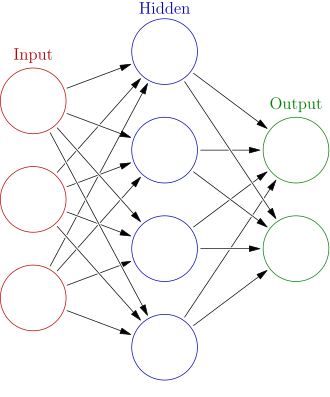
\includegraphics[width=0.6\linewidth]{figures/fig01-NeuralNetwork.png}
                \caption{Una rete neurale}
                \label{fig:placeholder}
            \end{figure}
    \end{columns}
\end{frame}

\begin{frame}
    \only<presentation>{
        \frametitle{Il machine learning (6)}
    }
    
    \begin{block}{}
        Il \textbf{\structure{deep learning}} (\textbf{\structure{DL}}) è una tecnica di IA che fa uso di una rete neurale profonda (\textbf{\structure{DDN}, \textit{Deep Neural Network}}), avente cioè più strati di elaborazione in grado di svolgere compiti complessi.
    \end{block}

    \vspace{\baselineskip}

    Il deep learning può essere considerato un sottoinsieme del machine learning in grado di operare su un dataset di grandi dimensioni e di apprendere in modo autonomo, senza necessità di addestramento da parte di una perspna esperta del problema affrontato , utilizzand algoritmi pià complessi rispetto al machine learning.
\end{frame}

\begin{frame}
    \only<presentation>{
        \frametitle{Il machine learning (7)}
    }

    Il deep learning è inoltre strettamente legato al concetto di \textbf{big data}, cioè insiemi di dati molto vasti, eterogenei e in continuo aggiornamento, provenienti da fonti diverse come social network, Internet delle cose (\textbf{IoT}, \textit{Internet of Things}), transazioni online, immagini o video diffusi in rete.

    \vspace{\baselineskip}

    Infatti gli algoritmi di deep learning, per funzionare efficacemente, hanno bisogno di grandi quantità di dati che consentano di sviluppare la capacità di apprendere, individuare schemi ricorrenti e generalizzare le conoscenza acquisite.
\end{frame}

\begin{frame}
    \only<presentation>{
        \frametitle{Il machine learning (8)}
    }

    \begin{block}{Esempio}
        Il machine learning e, a un livello più avanzato, le reti neurali e il deep learning possono essere applicati in ambito sanitario nel settore della \textbf{radiomica} (o \textit{radiomics}) che si occupa dell'analisi automatica delle immagini mediche, come radiografie, risonanze magnetiche o tomografie. Il sistema viene addestrato su milioni di immagini mediche etichettate (\textbf{labeling}, vedi \hl{[lezione con pag. 390]}), cioè giù valutate da personale medico specializzato, e impara a riconoscere automaticamente modelli visivi (\textbf{pattern}) associati a patologie, favorendo l'accuratezza e la rapidità delle diagnosi.
    \end{block}
\end{frame}

% -----

\subsection{Intelligenza Artificiale generativa}

\begin{frame}
    \only<presentation>{
        \frametitle{Intelligenza Artificiale generativa (1)}
    }

    L'\textbf{\structure{Intelligenza Artificiale generativa}} (\textbf{\structure{GenAI}}, \textit{Generative Artificial Intelligence}) è il settore dell'Intelligenza Artificiale che si occupa della creazione di nuovi contenuti originali e creativi, non solo testi ma anche immagini, suoni, video e codice software.

    \vspace{\baselineskip}

    I \textbf{\structure{chatbot}} sono sistemi di Intelligenza Artificiale generativa che, grazie all'addestramento effettuato su grandi quantità di dati, sono in grado di comprendere le richieste dell'utente e di rispondere ai comandi e domande (\textbf{prompt}), simulando una conversazione (in inglese: \textit{chat}) n linguaggio naturale.
\end{frame}

\begin{frame}
    \only<presentation>{
        \frametitle{Intelligenza Artificiale generativa (2)}
    }

    \begin{block}{Esempio}
        Si possono generare velocemente \textbf{contenuti standard}, come manuali tecnici, e-mail commerciali da inviare a un grande numero di indirizzi o annunci pubblicitari.

        \vspace{\baselineskip}

        Anche le \textbf{pagine Web} di un sito possono essere create un modo automatico e rapido, facilitandone l'aggiornamento e la presentazione coinvolgente per l'utente.

        \vspace{\baselineskip}

        Per una piattaforma di \textbf{e-commerce} con un grande numero di prodotti in vendita si possono generare descrizioni, sintesi delle recensioni di utenti, immagini e video per ciascun prodotto da pubblicare sul sito Web.
    \end{block}
\end{frame}

% -----

\begin{frame}{Riferimenti e approfondimenti}
    \printbibliography
\end{frame}

% -----

\end{document}
